\section{BiLinear Discontinous finite elements}
In this research, the BLD basis functions are used only on the rectangular
cells. If the cells are arbitrary convex quadrilateral, the discretization may
not exist (the system of equations obtained may be ill-conditioned). The BLD basis 
functions defined on the following rectangular cell:
\begin{figure}[H]
  \centering
  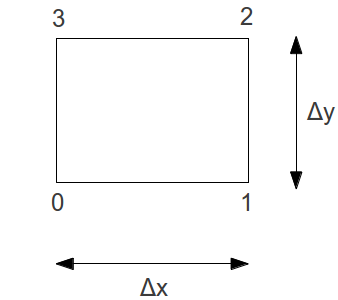
\includegraphics[width=0.2\textwidth]{./Spatial_discretizations/cell}
  \caption{Cell}
\end{figure}
are:
\begin{align}
  &b_0(x,y) = \frac{(dx-x)}{dx}\frac{(dy-y)}{dy}\\
  &b_1(x,y) = \frac{x}{dx}\frac{(dy-y)}{dy}\\
  &b_2(x,y) = \frac{x}{dx}\frac{y}{dy}\\
  &b_3(x,y) = \frac{(dx-x)}{dx}\frac{y}{dy}
\end{align}
with $x\in[0,dx]$ and $y\in[0,dy]$. On a square cell, the basis functions are
given in Figure (\ref{bld}):
\begin{figure}[H]
\centering    
\subfloat[First basis function]{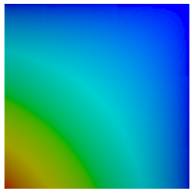
\includegraphics[width=0.25\textwidth]
  {./Spatial_discretizations/bld_1}}
\subfloat[Second basis function]{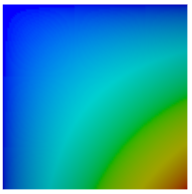
\includegraphics[width=0.25\textwidth]
  {./Spatial_discretizations/bld_2}}\\
\subfloat[Third basis function]{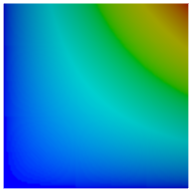
\includegraphics[width=0.25\textwidth]
  {./Spatial_discretizations/bld_3}}
\subfloat[Fourth basis function]{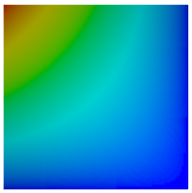
\includegraphics[width=0.25\textwidth]
  {./Spatial_discretizations/bld_4}}
\caption{BLD basis function}
\label{bld}
\end{figure}
Given these basis functions \crefrange{precomputed_1}{precomputed_5} can be
easily analytically computed on rectangular cells. 
